% Options for packages loaded elsewhere
\PassOptionsToPackage{unicode}{hyperref}
\PassOptionsToPackage{hyphens}{url}
%
\documentclass[
  8pt,
  ignorenonframetext,
]{beamer}
\usepackage{pgfpages}
\setbeamertemplate{caption}[numbered]
\setbeamertemplate{caption label separator}{: }
\setbeamercolor{caption name}{fg=normal text.fg}
\beamertemplatenavigationsymbolsempty
% Prevent slide breaks in the middle of a paragraph
\widowpenalties 1 10000
\raggedbottom
\setbeamertemplate{part page}{
  \centering
  \begin{beamercolorbox}[sep=16pt,center]{part title}
    \usebeamerfont{part title}\insertpart\par
  \end{beamercolorbox}
}
\setbeamertemplate{section page}{
  \centering
  \begin{beamercolorbox}[sep=12pt,center]{section title}
    \usebeamerfont{section title}\insertsection\par
  \end{beamercolorbox}
}
\setbeamertemplate{subsection page}{
  \centering
  \begin{beamercolorbox}[sep=8pt,center]{subsection title}
    \usebeamerfont{subsection title}\insertsubsection\par
  \end{beamercolorbox}
}
\AtBeginPart{
  \frame{\partpage}
}
\AtBeginSection{
  \ifbibliography
  \else
    \frame{\sectionpage}
  \fi
}
\AtBeginSubsection{
  \frame{\subsectionpage}
}

\usepackage{amsmath,amssymb}
\usepackage{iftex}
\ifPDFTeX
  \usepackage[T1]{fontenc}
  \usepackage[utf8]{inputenc}
  \usepackage{textcomp} % provide euro and other symbols
\else % if luatex or xetex
  \usepackage{unicode-math}
  \defaultfontfeatures{Scale=MatchLowercase}
  \defaultfontfeatures[\rmfamily]{Ligatures=TeX,Scale=1}
\fi
\usepackage{lmodern}
\usetheme[]{Madrid}
\usecolortheme{seahorse}
\ifPDFTeX\else  
    % xetex/luatex font selection
\fi
% Use upquote if available, for straight quotes in verbatim environments
\IfFileExists{upquote.sty}{\usepackage{upquote}}{}
\IfFileExists{microtype.sty}{% use microtype if available
  \usepackage[]{microtype}
  \UseMicrotypeSet[protrusion]{basicmath} % disable protrusion for tt fonts
}{}
\makeatletter
\@ifundefined{KOMAClassName}{% if non-KOMA class
  \IfFileExists{parskip.sty}{%
    \usepackage{parskip}
  }{% else
    \setlength{\parindent}{0pt}
    \setlength{\parskip}{6pt plus 2pt minus 1pt}}
}{% if KOMA class
  \KOMAoptions{parskip=half}}
\makeatother
\usepackage{xcolor}
\newif\ifbibliography
\setlength{\emergencystretch}{3em} % prevent overfull lines
\setcounter{secnumdepth}{-\maxdimen} % remove section numbering

\usepackage{color}
\usepackage{fancyvrb}
\newcommand{\VerbBar}{|}
\newcommand{\VERB}{\Verb[commandchars=\\\{\}]}
\DefineVerbatimEnvironment{Highlighting}{Verbatim}{commandchars=\\\{\}}
% Add ',fontsize=\small' for more characters per line
\usepackage{framed}
\definecolor{shadecolor}{RGB}{241,243,245}
\newenvironment{Shaded}{\begin{snugshade}}{\end{snugshade}}
\newcommand{\AlertTok}[1]{\textcolor[rgb]{0.68,0.00,0.00}{#1}}
\newcommand{\AnnotationTok}[1]{\textcolor[rgb]{0.37,0.37,0.37}{#1}}
\newcommand{\AttributeTok}[1]{\textcolor[rgb]{0.40,0.45,0.13}{#1}}
\newcommand{\BaseNTok}[1]{\textcolor[rgb]{0.68,0.00,0.00}{#1}}
\newcommand{\BuiltInTok}[1]{\textcolor[rgb]{0.00,0.23,0.31}{#1}}
\newcommand{\CharTok}[1]{\textcolor[rgb]{0.13,0.47,0.30}{#1}}
\newcommand{\CommentTok}[1]{\textcolor[rgb]{0.37,0.37,0.37}{#1}}
\newcommand{\CommentVarTok}[1]{\textcolor[rgb]{0.37,0.37,0.37}{\textit{#1}}}
\newcommand{\ConstantTok}[1]{\textcolor[rgb]{0.56,0.35,0.01}{#1}}
\newcommand{\ControlFlowTok}[1]{\textcolor[rgb]{0.00,0.23,0.31}{\textbf{#1}}}
\newcommand{\DataTypeTok}[1]{\textcolor[rgb]{0.68,0.00,0.00}{#1}}
\newcommand{\DecValTok}[1]{\textcolor[rgb]{0.68,0.00,0.00}{#1}}
\newcommand{\DocumentationTok}[1]{\textcolor[rgb]{0.37,0.37,0.37}{\textit{#1}}}
\newcommand{\ErrorTok}[1]{\textcolor[rgb]{0.68,0.00,0.00}{#1}}
\newcommand{\ExtensionTok}[1]{\textcolor[rgb]{0.00,0.23,0.31}{#1}}
\newcommand{\FloatTok}[1]{\textcolor[rgb]{0.68,0.00,0.00}{#1}}
\newcommand{\FunctionTok}[1]{\textcolor[rgb]{0.28,0.35,0.67}{#1}}
\newcommand{\ImportTok}[1]{\textcolor[rgb]{0.00,0.46,0.62}{#1}}
\newcommand{\InformationTok}[1]{\textcolor[rgb]{0.37,0.37,0.37}{#1}}
\newcommand{\KeywordTok}[1]{\textcolor[rgb]{0.00,0.23,0.31}{\textbf{#1}}}
\newcommand{\NormalTok}[1]{\textcolor[rgb]{0.00,0.23,0.31}{#1}}
\newcommand{\OperatorTok}[1]{\textcolor[rgb]{0.37,0.37,0.37}{#1}}
\newcommand{\OtherTok}[1]{\textcolor[rgb]{0.00,0.23,0.31}{#1}}
\newcommand{\PreprocessorTok}[1]{\textcolor[rgb]{0.68,0.00,0.00}{#1}}
\newcommand{\RegionMarkerTok}[1]{\textcolor[rgb]{0.00,0.23,0.31}{#1}}
\newcommand{\SpecialCharTok}[1]{\textcolor[rgb]{0.37,0.37,0.37}{#1}}
\newcommand{\SpecialStringTok}[1]{\textcolor[rgb]{0.13,0.47,0.30}{#1}}
\newcommand{\StringTok}[1]{\textcolor[rgb]{0.13,0.47,0.30}{#1}}
\newcommand{\VariableTok}[1]{\textcolor[rgb]{0.07,0.07,0.07}{#1}}
\newcommand{\VerbatimStringTok}[1]{\textcolor[rgb]{0.13,0.47,0.30}{#1}}
\newcommand{\WarningTok}[1]{\textcolor[rgb]{0.37,0.37,0.37}{\textit{#1}}}

\providecommand{\tightlist}{%
  \setlength{\itemsep}{0pt}\setlength{\parskip}{0pt}}\usepackage{longtable,booktabs,array}
\usepackage{calc} % for calculating minipage widths
\usepackage{caption}
% Make caption package work with longtable
\makeatletter
\def\fnum@table{\tablename~\thetable}
\makeatother
\usepackage{graphicx}
\makeatletter
\newsavebox\pandoc@box
\newcommand*\pandocbounded[1]{% scales image to fit in text height/width
  \sbox\pandoc@box{#1}%
  \Gscale@div\@tempa{\textheight}{\dimexpr\ht\pandoc@box+\dp\pandoc@box\relax}%
  \Gscale@div\@tempb{\linewidth}{\wd\pandoc@box}%
  \ifdim\@tempb\p@<\@tempa\p@\let\@tempa\@tempb\fi% select the smaller of both
  \ifdim\@tempa\p@<\p@\scalebox{\@tempa}{\usebox\pandoc@box}%
  \else\usebox{\pandoc@box}%
  \fi%
}
% Set default figure placement to htbp
\def\fps@figure{htbp}
\makeatother

\makeatletter
\@ifpackageloaded{caption}{}{\usepackage{caption}}
\AtBeginDocument{%
\ifdefined\contentsname
  \renewcommand*\contentsname{Table of contents}
\else
  \newcommand\contentsname{Table of contents}
\fi
\ifdefined\listfigurename
  \renewcommand*\listfigurename{List of Figures}
\else
  \newcommand\listfigurename{List of Figures}
\fi
\ifdefined\listtablename
  \renewcommand*\listtablename{List of Tables}
\else
  \newcommand\listtablename{List of Tables}
\fi
\ifdefined\figurename
  \renewcommand*\figurename{Figure}
\else
  \newcommand\figurename{Figure}
\fi
\ifdefined\tablename
  \renewcommand*\tablename{Table}
\else
  \newcommand\tablename{Table}
\fi
}
\@ifpackageloaded{float}{}{\usepackage{float}}
\floatstyle{ruled}
\@ifundefined{c@chapter}{\newfloat{codelisting}{h}{lop}}{\newfloat{codelisting}{h}{lop}[chapter]}
\floatname{codelisting}{Listing}
\newcommand*\listoflistings{\listof{codelisting}{List of Listings}}
\makeatother
\makeatletter
\makeatother
\makeatletter
\@ifpackageloaded{caption}{}{\usepackage{caption}}
\@ifpackageloaded{subcaption}{}{\usepackage{subcaption}}
\makeatother

\usepackage{bookmark}

\IfFileExists{xurl.sty}{\usepackage{xurl}}{} % add URL line breaks if available
\urlstyle{same} % disable monospaced font for URLs
\hypersetup{
  pdftitle={R Assignment 1 - Summer},
  pdfauthor={Sanmesh Sanjay Shintre},
  hidelinks,
  pdfcreator={LaTeX via pandoc}}


\title{R Assignment 1 - Summer}
\author{Sanmesh Sanjay Shintre}
\date{}

\begin{document}
\frame{\titlepage}

\renewcommand*\contentsname{Table of contents}
\begin{frame}[allowframebreaks]
  \frametitle{Table of contents}
  \setcounter{tocdepth}{3}
  \tableofcontents
\end{frame}

\section{Use data.table to read in the
data}\label{use-data.table-to-read-in-the-data}

\begin{frame}[fragile]{Use data.table to read in the data}
\begin{Shaded}
\begin{Highlighting}[]
\FunctionTok{library}\NormalTok{(data.table)}
\FunctionTok{library}\NormalTok{(ggplot2)  }
\FunctionTok{library}\NormalTok{(knitr)}
\FunctionTok{library}\NormalTok{(dplyr)}

\CommentTok{\#Loading the datasets }
\NormalTok{dt\_india }\OtherTok{\textless{}{-}} \FunctionTok{fread}\NormalTok{(}\StringTok{"indicators\_ind.csv"}\NormalTok{)[}\SpecialCharTok{{-}}\DecValTok{1}\NormalTok{,]}
\NormalTok{dt\_are }\OtherTok{\textless{}{-}} \FunctionTok{fread}\NormalTok{(}\StringTok{"indicators\_are.csv"}\NormalTok{)[}\SpecialCharTok{{-}}\DecValTok{1}\NormalTok{,]}
\NormalTok{dt\_usa }\OtherTok{\textless{}{-}} \FunctionTok{fread}\NormalTok{(}\StringTok{"indicators\_usa.csv"}\NormalTok{)[}\SpecialCharTok{{-}}\DecValTok{1}\NormalTok{,]}
\end{Highlighting}
\end{Shaded}

\begin{itemize}
\item
  Loading the packages required.
\item
  Loaded the dataset using fread for 3 countries.
\end{itemize}
\end{frame}

\section{Assign the correct class to the
variables}\label{assign-the-correct-class-to-the-variables}

\begin{frame}[fragile]{Assign the correct class to the variables}
\begin{Shaded}
\begin{Highlighting}[]
\FunctionTok{options}\NormalTok{(}\AttributeTok{width =} \DecValTok{70}\NormalTok{)}
\NormalTok{dt\_india[, }\StringTok{\textasciigrave{}}\AttributeTok{:=}\StringTok{\textasciigrave{}}\NormalTok{(}
  \StringTok{\textasciigrave{}}\AttributeTok{Country Name}\StringTok{\textasciigrave{}} \OtherTok{=} \FunctionTok{as.factor}\NormalTok{(}\StringTok{\textasciigrave{}}\AttributeTok{Country Name}\StringTok{\textasciigrave{}}\NormalTok{),}
  \StringTok{\textasciigrave{}}\AttributeTok{Country ISO3}\StringTok{\textasciigrave{}} \OtherTok{=} \FunctionTok{as.factor}\NormalTok{(}\StringTok{\textasciigrave{}}\AttributeTok{Country ISO3}\StringTok{\textasciigrave{}}\NormalTok{),}
  \StringTok{\textasciigrave{}}\AttributeTok{Indicator Name}\StringTok{\textasciigrave{}} \OtherTok{=} \FunctionTok{as.factor}\NormalTok{(}\StringTok{\textasciigrave{}}\AttributeTok{Indicator Name}\StringTok{\textasciigrave{}}\NormalTok{),}
  \StringTok{\textasciigrave{}}\AttributeTok{Indicator Code}\StringTok{\textasciigrave{}} \OtherTok{=} \FunctionTok{as.factor}\NormalTok{(}\StringTok{\textasciigrave{}}\AttributeTok{Indicator Code}\StringTok{\textasciigrave{}}\NormalTok{),}
  \AttributeTok{Year =} \FunctionTok{as.integer}\NormalTok{(Year),}
  \AttributeTok{Value =} \FunctionTok{as.numeric}\NormalTok{(Value)}
\NormalTok{)]}
\NormalTok{dt\_are[, }\StringTok{\textasciigrave{}}\AttributeTok{:=}\StringTok{\textasciigrave{}}\NormalTok{(}
  \StringTok{\textasciigrave{}}\AttributeTok{Country Name}\StringTok{\textasciigrave{}} \OtherTok{=} \FunctionTok{as.factor}\NormalTok{(}\StringTok{\textasciigrave{}}\AttributeTok{Country Name}\StringTok{\textasciigrave{}}\NormalTok{),}
  \StringTok{\textasciigrave{}}\AttributeTok{Country ISO3}\StringTok{\textasciigrave{}} \OtherTok{=} \FunctionTok{as.factor}\NormalTok{(}\StringTok{\textasciigrave{}}\AttributeTok{Country ISO3}\StringTok{\textasciigrave{}}\NormalTok{),}
  \StringTok{\textasciigrave{}}\AttributeTok{Indicator Name}\StringTok{\textasciigrave{}} \OtherTok{=} \FunctionTok{as.factor}\NormalTok{(}\StringTok{\textasciigrave{}}\AttributeTok{Indicator Name}\StringTok{\textasciigrave{}}\NormalTok{),}
  \StringTok{\textasciigrave{}}\AttributeTok{Indicator Code}\StringTok{\textasciigrave{}} \OtherTok{=} \FunctionTok{as.factor}\NormalTok{(}\StringTok{\textasciigrave{}}\AttributeTok{Indicator Code}\StringTok{\textasciigrave{}}\NormalTok{),}
  \AttributeTok{Year =} \FunctionTok{as.integer}\NormalTok{(Year),}
  \AttributeTok{Value =} \FunctionTok{as.numeric}\NormalTok{(Value)}
\NormalTok{)]}
\NormalTok{dt\_usa[, }\StringTok{\textasciigrave{}}\AttributeTok{:=}\StringTok{\textasciigrave{}}\NormalTok{(}
  \StringTok{\textasciigrave{}}\AttributeTok{Country Name}\StringTok{\textasciigrave{}} \OtherTok{=} \FunctionTok{as.factor}\NormalTok{(}\StringTok{\textasciigrave{}}\AttributeTok{Country Name}\StringTok{\textasciigrave{}}\NormalTok{),}
  \StringTok{\textasciigrave{}}\AttributeTok{Country ISO3}\StringTok{\textasciigrave{}} \OtherTok{=} \FunctionTok{as.factor}\NormalTok{(}\StringTok{\textasciigrave{}}\AttributeTok{Country ISO3}\StringTok{\textasciigrave{}}\NormalTok{),}
  \StringTok{\textasciigrave{}}\AttributeTok{Indicator Name}\StringTok{\textasciigrave{}} \OtherTok{=} \FunctionTok{as.factor}\NormalTok{(}\StringTok{\textasciigrave{}}\AttributeTok{Indicator Name}\StringTok{\textasciigrave{}}\NormalTok{),}
  \StringTok{\textasciigrave{}}\AttributeTok{Indicator Code}\StringTok{\textasciigrave{}} \OtherTok{=} \FunctionTok{as.factor}\NormalTok{(}\StringTok{\textasciigrave{}}\AttributeTok{Indicator Code}\StringTok{\textasciigrave{}}\NormalTok{),}
  \AttributeTok{Year =} \FunctionTok{as.integer}\NormalTok{(Year),}
  \AttributeTok{Value =} \FunctionTok{as.numeric}\NormalTok{(Value)}
\NormalTok{)]}
\end{Highlighting}
\end{Shaded}
\end{frame}

\begin{frame}[fragile]{Combining 3 datasets}
\phantomsection\label{combining-3-datasets}
\begin{Shaded}
\begin{Highlighting}[]
\NormalTok{dt\_all }\OtherTok{\textless{}{-}} \FunctionTok{rbindlist}\NormalTok{(}\FunctionTok{list}\NormalTok{(dt\_india, dt\_are, dt\_usa)}
\NormalTok{                    , }\AttributeTok{use.names =} \ConstantTok{TRUE}\NormalTok{, }\AttributeTok{fill =} \ConstantTok{TRUE}\NormalTok{)}
\end{Highlighting}
\end{Shaded}

\begin{itemize}
\tightlist
\item
  Assigned the correct class for each of the column of dataset for
  respective countries.
\item
  Such as integer and numeric for Year and Value respectively.
\item
  Combined 3 datasets into one single dataset using rbindlist().
\end{itemize}
\end{frame}

\section{Data Exploration}\label{data-exploration}

\begin{frame}[fragile]{Data Exploration}
\begin{Shaded}
\begin{Highlighting}[]
\NormalTok{dt\_all[, .N, by }\OtherTok{=}\NormalTok{ .(}\StringTok{\textasciigrave{}}\AttributeTok{Country Name}\StringTok{\textasciigrave{}}\NormalTok{, }
                    \StringTok{\textasciigrave{}}\AttributeTok{Indicator Name}\StringTok{\textasciigrave{}}\NormalTok{)][, .N, by }\OtherTok{=} \StringTok{\textasciigrave{}}\AttributeTok{Country Name}\StringTok{\textasciigrave{}}\NormalTok{]}
\end{Highlighting}
\end{Shaded}

\begin{verbatim}
           Country Name     N
                 <fctr> <int>
1:                India  3633
2: United Arab Emirates  1921
3:        United States  2000
\end{verbatim}

\begin{Shaded}
\begin{Highlighting}[]
\NormalTok{common\_indicators }\OtherTok{\textless{}{-}} \FunctionTok{Reduce}\NormalTok{(intersect, }\FunctionTok{list}\NormalTok{(}
  \FunctionTok{unique}\NormalTok{(dt\_india}\SpecialCharTok{$}\StringTok{\textasciigrave{}}\AttributeTok{Indicator Name}\StringTok{\textasciigrave{}}\NormalTok{),}
  \FunctionTok{unique}\NormalTok{(dt\_are}\SpecialCharTok{$}\StringTok{\textasciigrave{}}\AttributeTok{Indicator Name}\StringTok{\textasciigrave{}}\NormalTok{),}
  \FunctionTok{unique}\NormalTok{(dt\_usa}\SpecialCharTok{$}\StringTok{\textasciigrave{}}\AttributeTok{Indicator Name}\StringTok{\textasciigrave{}}\NormalTok{)}
\NormalTok{))}
\FunctionTok{length}\NormalTok{(common\_indicators)  }
\end{Highlighting}
\end{Shaded}

\begin{verbatim}
[1] 1739
\end{verbatim}

\begin{itemize}
\item
  Taking the common indicators from dt\_all to common\_indicators.
\item
  Printing the number of common\_indicators in the dataset.
\end{itemize}
\end{frame}

\section{Data Exploration and plots}\label{data-exploration-and-plots}

\begin{frame}[fragile]{Data Exploration and plots}
\begin{Shaded}
\begin{Highlighting}[]
\NormalTok{indicator\_counts }\OtherTok{\textless{}{-}}\NormalTok{ dt\_all[, .N, by }\OtherTok{=}\NormalTok{ .(}\StringTok{\textasciigrave{}}\AttributeTok{Country Name}\StringTok{\textasciigrave{}}\NormalTok{, }\StringTok{\textasciigrave{}}\AttributeTok{Indicator Name}\StringTok{\textasciigrave{}}\NormalTok{)][, .N, by }\OtherTok{=} \StringTok{\textasciigrave{}}\AttributeTok{Country Name}\StringTok{\textasciigrave{}}\NormalTok{]}

\NormalTok{top\_indicators\_overall }\OtherTok{\textless{}{-}}\NormalTok{ dt\_all }\SpecialCharTok{\%\textgreater{}\%}
  \FunctionTok{group\_by}\NormalTok{(}\StringTok{\textasciigrave{}}\AttributeTok{Indicator Name}\StringTok{\textasciigrave{}}\NormalTok{) }\SpecialCharTok{\%\textgreater{}\%}
  \FunctionTok{summarise}\NormalTok{(}\AttributeTok{Count =} \FunctionTok{n}\NormalTok{(), }\AttributeTok{.groups =} \StringTok{"drop"}\NormalTok{) }\SpecialCharTok{\%\textgreater{}\%}
  \FunctionTok{slice\_max}\NormalTok{(}\AttributeTok{order\_by =}\NormalTok{ Count, }\AttributeTok{n =} \DecValTok{15}\NormalTok{)}
\end{Highlighting}
\end{Shaded}

\begin{itemize}
\item
  Count \textbf{how many indicators} each country has: two‐step grouping
  with .N.
\item
  Prepare two exploratory outputs:

  \begin{enumerate}
  \item
    \textbf{indicator\_counts} (per country)
  \item
    \textbf{top\_indicators\_overall} (top 15 by frequency)
  \end{enumerate}
\end{itemize}
\end{frame}

\section{Data Analysis using data.table (with
keyby)}\label{data-analysis-using-data.table-with-keyby}

\begin{frame}[fragile]{Data Analysis using data.table (with keyby)}
\begin{Shaded}
\begin{Highlighting}[]
\NormalTok{dt\_filtered }\OtherTok{\textless{}{-}}\NormalTok{ dt\_all[}\StringTok{\textasciigrave{}}\AttributeTok{Indicator Name}\StringTok{\textasciigrave{}} \SpecialCharTok{\%in\%}\NormalTok{ common\_indicators]}
\NormalTok{dt\_migration\_summary }\OtherTok{\textless{}{-}}\NormalTok{ dt\_filtered[}
  \StringTok{\textasciigrave{}}\AttributeTok{Indicator Name}\StringTok{\textasciigrave{}} \SpecialCharTok{==} \StringTok{"Net migration"}\NormalTok{,}
\NormalTok{  .(}\AttributeTok{Average\_Migration =} \FunctionTok{mean}\NormalTok{(Value, }\AttributeTok{na.rm =} \ConstantTok{TRUE}\NormalTok{)),}
\NormalTok{  keyby }\OtherTok{=}\NormalTok{ .(Year, }\StringTok{\textasciigrave{}}\AttributeTok{Country Name}\StringTok{\textasciigrave{}}\NormalTok{)}
\NormalTok{]}
\NormalTok{dt\_fuel\_exports }\OtherTok{\textless{}{-}}\NormalTok{ dt\_filtered[}\StringTok{\textasciigrave{}}\AttributeTok{Indicator Name}\StringTok{\textasciigrave{}} \SpecialCharTok{==}
                                 \StringTok{"Fuel exports (\% of merchandise exports)"}\NormalTok{]}
\NormalTok{dt\_fuel\_summary }\OtherTok{\textless{}{-}}\NormalTok{ dt\_fuel\_exports[,.(}
    \AttributeTok{Avg\_Export =} \FunctionTok{mean}\NormalTok{(Value, }\AttributeTok{na.rm =} \ConstantTok{TRUE}\NormalTok{),}
    \AttributeTok{SD\_Export =} \FunctionTok{sd}\NormalTok{(Value, }\AttributeTok{na.rm =} \ConstantTok{TRUE}\NormalTok{),}
    \AttributeTok{Min =} \FunctionTok{min}\NormalTok{(Value, }\AttributeTok{na.rm =} \ConstantTok{TRUE}\NormalTok{),}
    \AttributeTok{Max =} \FunctionTok{max}\NormalTok{(Value, }\AttributeTok{na.rm =} \ConstantTok{TRUE}\NormalTok{),}
    \AttributeTok{Observations =}\NormalTok{ .N}
\NormalTok{  ),keyby }\OtherTok{=} \StringTok{\textasciigrave{}}\AttributeTok{Country Name}\StringTok{\textasciigrave{}}
\NormalTok{]}
\end{Highlighting}
\end{Shaded}
\end{frame}

\begin{frame}[fragile]{Data Analysis using data.table (with keyby)}
\phantomsection\label{data-analysis-using-data.table-with-keyby-1}
\begin{Shaded}
\begin{Highlighting}[]
\NormalTok{dt\_fuel\_summary}
\end{Highlighting}
\end{Shaded}

\begin{verbatim}
Key: <Country Name>
           Country Name Avg_Export SD_Export       Min      Max
                 <fctr>      <num>     <num>     <num>    <num>
1:                India   6.845227  7.041200 0.2473565 21.75247
2: United Arab Emirates  56.501599 24.217227 7.2975111 94.91210
3:        United States   5.571262  4.617027 1.5251860 21.41017
   Observations
          <int>
1:          186
2:           93
3:          186
\end{verbatim}

\begin{itemize}
\item
  \textbf{Filter} to only the common\_indicators.
\item
  Use \textbf{keyby} to efficiently compute:

  \begin{itemize}
  \tightlist
  \item
    \textbf{Average Net Migration} by Year \& Country
  \item
    \textbf{Fuel Exports} summary stats by Country
  \end{itemize}
\end{itemize}
\end{frame}

\section{Plots}\label{plots}

\begin{frame}[fragile]{Plot 1 of Analysis}
\phantomsection\label{plot-1-of-analysis}
\begin{Shaded}
\begin{Highlighting}[]
\FunctionTok{ggplot}\NormalTok{(indicator\_counts, }\FunctionTok{aes}\NormalTok{(}\AttributeTok{x =} \StringTok{\textasciigrave{}}\AttributeTok{Country Name}\StringTok{\textasciigrave{}}\NormalTok{, }\AttributeTok{y =}\NormalTok{ N, }\AttributeTok{fill =} \StringTok{\textasciigrave{}}\AttributeTok{Country Name}\StringTok{\textasciigrave{}}\NormalTok{)) }\SpecialCharTok{+}
  \FunctionTok{geom\_col}\NormalTok{(}\AttributeTok{width =} \FloatTok{0.6}\NormalTok{) }\SpecialCharTok{+}
  \FunctionTok{theme\_minimal}\NormalTok{() }\SpecialCharTok{+}
  \FunctionTok{labs}\NormalTok{(}
    \AttributeTok{title =} \StringTok{"Number of Unique Indicators per Country"}\NormalTok{,}
    \AttributeTok{x =} \StringTok{"Country"}\NormalTok{,}
    \AttributeTok{y =} \StringTok{"Number of Indicators"}
\NormalTok{  ) }\SpecialCharTok{+}
  \FunctionTok{theme}\NormalTok{(}\AttributeTok{legend.position =} \StringTok{"none"}\NormalTok{)}
\end{Highlighting}
\end{Shaded}

\pandocbounded{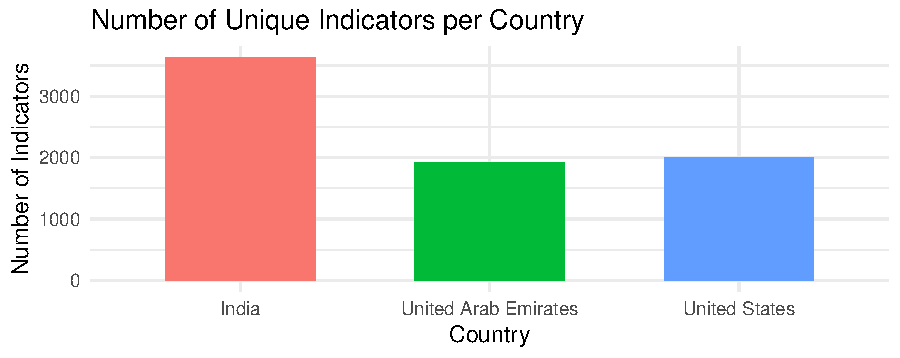
\includegraphics[keepaspectratio]{Assignment1_files/figure-beamer/unnamed-chunk-8-1.pdf}}
\end{frame}

\begin{frame}[fragile]{Plot 2 of Analysis}
\phantomsection\label{plot-2-of-analysis}
\begin{Shaded}
\begin{Highlighting}[]
\FunctionTok{ggplot}\NormalTok{(top\_indicators\_overall, }\FunctionTok{aes}\NormalTok{(}\AttributeTok{x =} \FunctionTok{reorder}\NormalTok{(}\StringTok{\textasciigrave{}}\AttributeTok{Indicator Name}\StringTok{\textasciigrave{}}\NormalTok{, Count), }\AttributeTok{y =}\NormalTok{ Count)) }\SpecialCharTok{+}
  \FunctionTok{geom\_col}\NormalTok{(}\AttributeTok{fill =} \StringTok{"steelblue"}\NormalTok{) }\SpecialCharTok{+}
  \FunctionTok{coord\_flip}\NormalTok{() }\SpecialCharTok{+}
  \FunctionTok{labs}\NormalTok{(}
    \AttributeTok{title =} \StringTok{"Top 15 Most Common Indicators in Dataset"}\NormalTok{,}
    \AttributeTok{x =} \StringTok{"Indicator"}\NormalTok{,}
    \AttributeTok{y =} \StringTok{"Observation Count"}
\NormalTok{  ) }\SpecialCharTok{+}
  \FunctionTok{theme\_minimal}\NormalTok{(}\AttributeTok{base\_size =} \DecValTok{8}\NormalTok{)}
\end{Highlighting}
\end{Shaded}

\pandocbounded{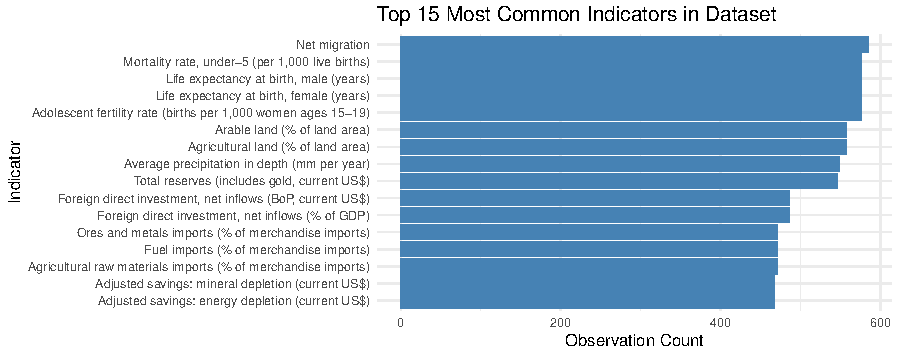
\includegraphics[keepaspectratio]{Assignment1_files/figure-beamer/unnamed-chunk-9-1.pdf}}
\end{frame}

\begin{frame}[fragile]{Plot 3 of Analysis}
\phantomsection\label{plot-3-of-analysis}
\begin{Shaded}
\begin{Highlighting}[]
\FunctionTok{ggplot}\NormalTok{(dt\_migration\_summary, }\FunctionTok{aes}\NormalTok{(}\AttributeTok{x =}\NormalTok{ Year, }\AttributeTok{y =}\NormalTok{ Average\_Migration, }
                                 \AttributeTok{color =} \StringTok{\textasciigrave{}}\AttributeTok{Country Name}\StringTok{\textasciigrave{}}\NormalTok{)) }\SpecialCharTok{+}
  \FunctionTok{geom\_line}\NormalTok{(}\AttributeTok{linewidth =} \FloatTok{1.2}\NormalTok{) }\SpecialCharTok{+}
  \FunctionTok{theme\_minimal}\NormalTok{() }\SpecialCharTok{+}
  \FunctionTok{labs}\NormalTok{(}
    \AttributeTok{title =} \StringTok{"Average Net Migration Over Time"}\NormalTok{,}
    \AttributeTok{x =} \StringTok{"Year"}\NormalTok{,}
    \AttributeTok{y =} \StringTok{"Average Migration"}\NormalTok{,}
    \AttributeTok{color =} \StringTok{"Country"}
\NormalTok{  )}
\end{Highlighting}
\end{Shaded}

\pandocbounded{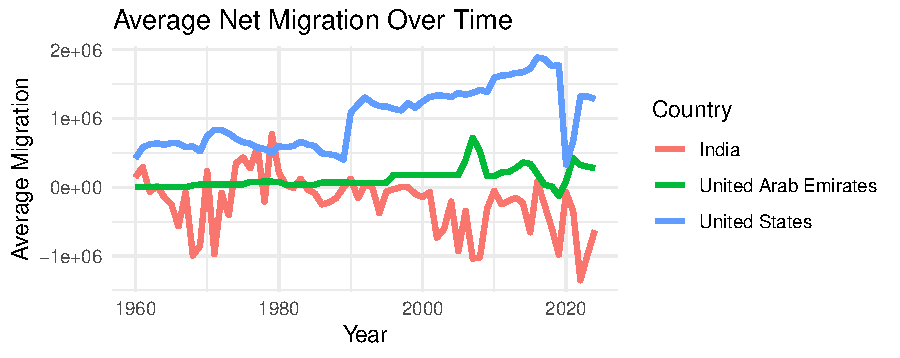
\includegraphics[keepaspectratio]{Assignment1_files/figure-beamer/unnamed-chunk-10-1.pdf}}
\end{frame}

\begin{frame}[fragile]{Plot 4 of Analysis}
\phantomsection\label{plot-4-of-analysis}
\begin{Shaded}
\begin{Highlighting}[]
\FunctionTok{ggplot}\NormalTok{(dt\_fuel\_summary, }\FunctionTok{aes}\NormalTok{(}\AttributeTok{x =} \StringTok{\textasciigrave{}}\AttributeTok{Country Name}\StringTok{\textasciigrave{}}\NormalTok{, }\AttributeTok{y =}\NormalTok{ Avg\_Export, }
                            \AttributeTok{fill =} \StringTok{\textasciigrave{}}\AttributeTok{Country Name}\StringTok{\textasciigrave{}}\NormalTok{)) }\SpecialCharTok{+}
  \FunctionTok{geom\_col}\NormalTok{(}\AttributeTok{width =} \FloatTok{0.6}\NormalTok{) }\SpecialCharTok{+}
  \FunctionTok{theme\_minimal}\NormalTok{() }\SpecialCharTok{+}
  \FunctionTok{labs}\NormalTok{(}
    \AttributeTok{title =} \StringTok{"Average Fuel Exports (\% of Merchandise Exports)"}\NormalTok{,}
    \AttributeTok{x =} \StringTok{"Country"}\NormalTok{, }\AttributeTok{y =} \StringTok{"Average \% of Fuel Exports"}
\NormalTok{  ) }\SpecialCharTok{+}
  \FunctionTok{theme}\NormalTok{(}\AttributeTok{legend.position =} \StringTok{"none"}\NormalTok{)}
\end{Highlighting}
\end{Shaded}

\pandocbounded{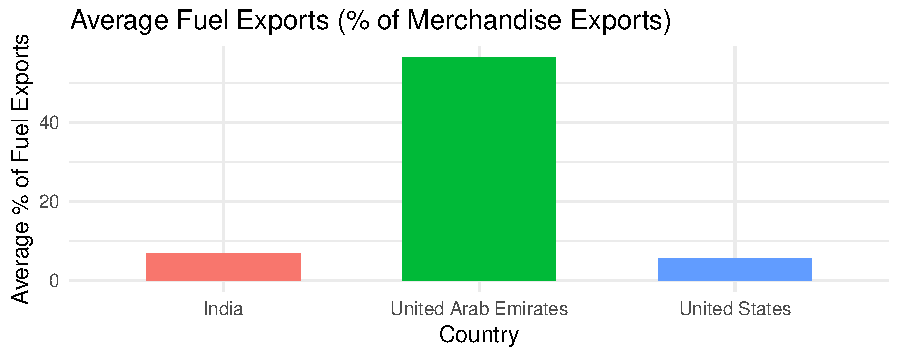
\includegraphics[keepaspectratio]{Assignment1_files/figure-beamer/unnamed-chunk-11-1.pdf}}
\end{frame}




\end{document}
